O presente trabalho busca propor um modelo numérico capaz de prever os perfis de
temperatura e pressão no interior de uma amostra de concreto refratário sujeito
ao aquecimento. Para tanto é fundamental o uso de experimentos para a obtenção
das propriedades necessárias ao modelo bem como ensaios que permitam a validação
do mesmo. Assim, a presente seção apresenta o levantamento das características
necessárias ao modelamento bem como os testes para validação do modelo. Além
disso há uma seção específica (Seção \ref{mat:fenics}) que descreve o modelo
matemático bem como a sua implementação em Python usando o pacote FEniCS. É
porém de fundamental importância determinar uma composição que será utilizada
e modelada, e portanto é a seção que inicia o presente capítulo.

\section{Composição de Concreto Refratário Aluminoso}

        
\section{Caracterização Experimental}\label{mat:exp}
As propriedades fundamentais para o modelo são

\begin{itemize}
\item Permeabilidade ($\kappa$)
\item Condutividade Térmica ($\lambda$)
\item Densidade ($\rho$)
\item Calor Específico ($\C_p$)
\item Água liberada por desidratação ($w_d$)
\end{itemize}

Além disso, as curvas de sorção isotérmica também se faz necessária, porém,
devido a ampla dificuldade em mensurá-la, o presente trabalho adotará a curva
padrão para concretos refratários reportada por Gong et al\cite{Gong1995a}. Além
de tais propriedades ensaios de Porosidade Aparente ($n_a$), e de Resistência
Mecânica também foram realizados para avaliar a suas relações com as
propriedades obtidas.

    \subsection{Porosidade e Densidade Aparente}\label{mat:porosidade}
    A porosidade e a densidade aparente dos materiais foram obtidas através do
    método de imersão usando o princípio de Arquimedes em corpos de prova
    tratados previamente a temperaturas de 30$^\circ$C, 110$^\circ$C,
    150$^\circ$C e 200$^\circ$C, 250$^\circ$C e 350$^\circ$C. Devido a
    possibilidade de hidratação do cimento, o fluído de imersão utilizado foi
    querosene (conforme recomendado pela norma ASTM C 830) e os valores de
    porosidade aparente, $n_a$ e de densidade aparente, $\rho$, foram calculados
    conforme as Equações \ref{eq:PA} e \ref{eq:DA}, respectivamente.

    \begin{equation}
      \label{eq:PA}
      n_a (\%)= 100 \ \frac{P_u-P_s}{P_u-P_i}
    \end{equation}

    \begin{equation}
      \label{eq:DA}
      \rho = \frac{P_s}{P_s - P_i} \ \rho_f
    \end{equation}

    Onde $P_u$ é o peso a úmido, $P_s$ é o peso da amostra submerso no fluído,
    $P_s$ é o peso da amostra a seco e $\rho_f$ é a densidade do fluído (no
    caso a densidade da querosene, $rho_f = 820$ Kg/m$^3$). Cada valor foi obtido
    através da média de 5 amostras distintas.
    
    \subsection{Permeabilidade}\label{mat:perm}

    A permeabilidade dos materiais é uma medida da quantidade relativa dos poros
    abertos intercomunicantes no interior de uma amostra. Para tanto, uma forma
    de medi-la é através da velocidade de um fluído dado uma determinada queda
    de pressão entre as faces de uma amostra. No presente modelo se faz
    necessário obter a permeabilidade em diferentes temperaturas e portanto
    assume-se que a microestrutura do material pode ser aproximada pelo seu
    estado após um tratamento térmico em determinada temperatura, sendo a medida
    feita em temperatura ambiente, seguindo a Norma ASTM C577. As medidas são
    obtidas pela média de 3 amostras de formato cilíndrico com raio de 35mm e
    espessura de 25mm. Para a vedação do sistema se utiliza silicone além de um
    O-ring de borracha. O esquema é apresentado na Figura \ref{fig:perm}. O
    modelo utiliza a condutividade hidráulica que é obtida a partir da constante
    de permeabilidade Darciana ($k_1$) que representa as perdas de energia
    viscosa a baixas velocidades do ar. A medida porém também permite a medição do
    parâmetro $k_2$ devido a não linearidade da velocidade, caracterizada pela
    equação de Forchheimer, \ref{eq:forch}. Este segundo parâmetro diz respeito
    a perda de energia cinética a altas velocidades.

    \begin{equation}
      \label{eq:forch}
      \frac{P_e^2 - P_s^2}{2 \ P \ L} = \frac{\mu}{k_1} \ v_s + \frac{\rho}{k_2}v_s^2
    \end{equation}

    Onde $P_e$ e $P_s$ são as pressões absolutas na entrada e na saída da
    amostra medidas em atm, $P$ é a pressão a uma determinada vazão de ar, $L$ é a
    espessura da amostra em mm, $\mu$ é a viscosidade do ar medida em Pa s,
    $\rho$ é a densidade do ar g/cm$^3$ e $v_s$ é a velocidade do fluído em
    m/s.

    
    
  \begin{figure}[ht]
	\centering
	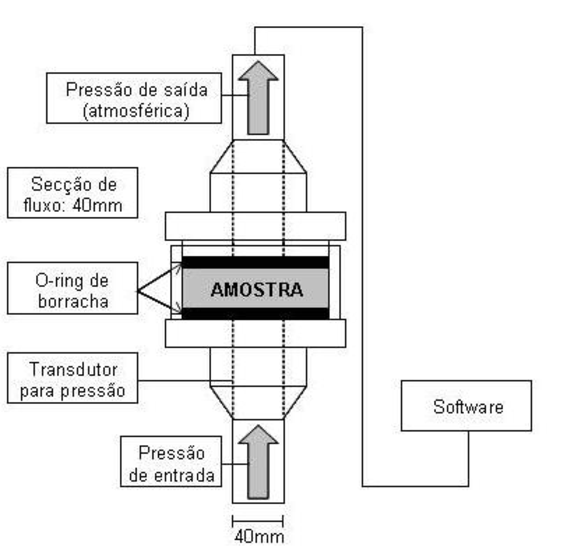
\includegraphics[width=9cm]{./figures/perm.pdf}
	\caption{Esquema de montagem do ensaio da medida de permeabilidade.  \label{fig:perm}}
  \end{figure}

   

    \subsection{Resistência Mecânica}\label{mat:rm}
    A resistência mecânica foi obtida através do ensaio de flecão em 3 pontos no
    mesmo intervalo de temperaturas usado para a obtenção da porosidade e
    densidade aparente, sendo realizados de acordo com a norma ASTM C133
    utilizando 5 corpos de prova no formato de paralelepípedos com dimensões de
    25 x 25 x 150 mm$^3$. O equipamento utilizado foi uma máquina de ensaios
    mecânicos universal (MTS, Modelo 810, USA) usando uma taxa de carregamento
    constante de 12.9 N.s$^{-1}$. O módulo de ruptura ($\sigma_f$) foi calculado
    pela Equação \ref{eq:modulo_rup}.

    \begin{equation}
      \label{eq:modulo_rup}
     \sigma_f = \frac{3 \ P \ L}{2 \ b \ d^2}
    \end{equation}

    Onde $P$, é a carga de ruptura medida em N, L é a distância  entre os
    apoios, fixa em 127 mm; b é a largura e d , a altura do corpo de prova,
    sendo todas as distâncias medidas em mm.
    
    \subsection{Termogravimetria (TGA)}\label{mat:TGA}
    
    Um dos principais ensaios para a simulação do processo de explosão durante o
    processo de secagem em escala laboratorial é o ensaio de termogravimetria. O
    sistema consiste em um forno com uma balança acoplada onde se mede a
    temperatura da amostra e do forno além da evolução do peso de uma amostra
    cilíndrica com 40 mm de diâmetro e 40 mm de altura. Os corpos são aquecidos
    após cura a 30$^\circ$C por 24 horas. Foram utilizadas taxas de aquecimento
    constantes de 2$^\circ$C.min$^{-1}$, 5$^\circ$C.min$^{-1}$ e
    20$^\circ$C.min$^{-1}$ no intervalo de 30$^\circ$C e 800$^\circ$C. A perda
    de massa e sua taxa temporal foram obtidas através das Equações
    \ref{eq:TGA_W} e \ref{eq:TGA_DTG}.

    \begin{equation}
      \label{eq:TGA_W}
      W = \left( \frac{M_0-M}{M_0-M_f} \right) \ 100
    \end{equation}

    \begin{equation}
      \label{eq:TGA_DTG}
      DTG = \frac{\partial W}{\partial t}
    \end{equation}

    Onde $M_0$ é a massa inicial da amostra, $M$ é a massa observada num
instante t, e $M_f$ corresponde à massa final da amostra (todas medidas em
gramas). $W$ é a perda de massa percentual, enquanto DTG é a taxa de perda de
massa (medida em \%.min$^{-1}$). A Figura \ref{fig:TGA} apresenta o esquema de
montagem do ensaio de termogravimetria.
    
 \begin{figure}[ht]
	\centering
	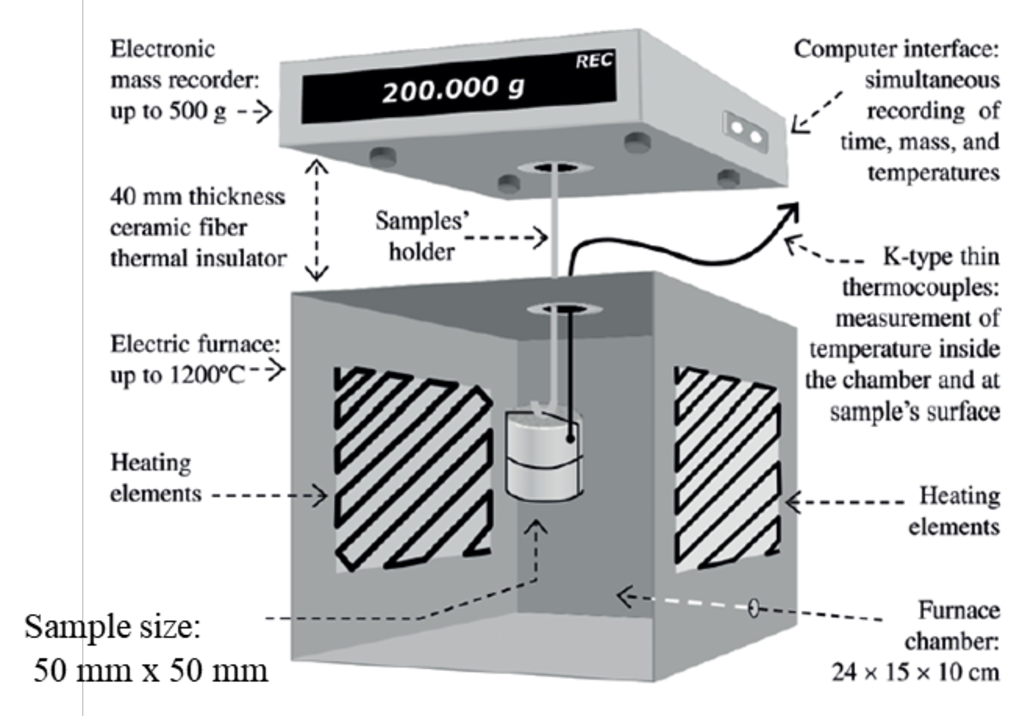
\includegraphics[width=9cm]{./figures/TGA.pdf}
	\caption{Esquema de montagem do ensaio de termogravimetria.  \label{fig:TGA}}
  \end{figure}



    \subsection{Condutividade Térmica e Calor Específico}\label{mat:condutividade}
    A condutividade térmica é obtida através do método do fio quente (com a
    configuração dos fios paralelos) através do
    equipamento Netzsch TCT 426. A medição se dá em um sistema de 3 tijolos com
    mesma composição dispostos um sobre os outros. Entalhes de 0.4mm são
    realizados nos tijolos usando uma retífica modelo Ferdimat T42 a fim de
    acomodar os fios do termopar.

    A técnica obtém o valor de condutividade através de uma estimativa baseada
    no tempo em que o calor gerado pelo fio quente (FQ) devido ao efeito Joule leva
    para ser percebido no termopar da amostra ($T_a$) em uma condição de equilíbrio
    térmico entra o conjunto de tijolos e o forno (através da medida de um
    termopar de referência $T_r$). Tal ensaio permite a obtenção do calor
    específico através da medida de difusividade térmica do material. A Figura \ref{fig:fio_quente}
    apresenta o {\it layout} do ensaio.

  \begin{figure}[ht]
	\centering
	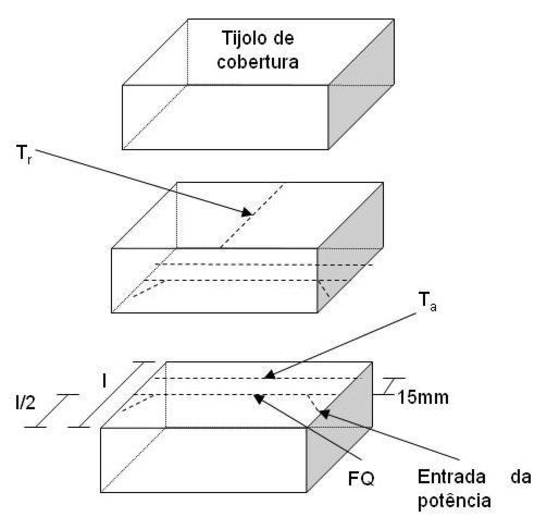
\includegraphics[width=9cm]{./figures/fio_quente.pdf}
	\caption{Esquema de montagem do ensaio da técnica de fio quente para obtenção
    da condutividade térmica e calor específico.  \label{fig:fio_quente}}
  \end{figure}


\section{Desenvolvimento do modelo em FEniCS}\label{mat:fenics}
     O presente trabalho baseia-se no modelo de Ba\v{z}ant
     \ref{sec:bazant}, assim a presente seção tem como objetivo apresentar a implementação
     do problema matemático através da plataforma FEniCS. Para tanto, é definida um caso a ser
     simulado, escolhe-se a geometria e as condições de contorno para melhor
     representar o problema físico. Em seguida é derivado o sistema de equações
     parciais diferenciais em sua forma forte, este é então convertido em sua forma
     fraca a qual é alimentada ao FEniCS e então realiza-se os calculos. Finalmente o script é
     apresentado e a rotina de pós processamento definida.

    \subsection{Caso Ilustrativo}\label{mat:caso}
    O caso a ser simulado é uma seção transversal em 2 dimensões de uma parede
    de concreto refratário com espessura de 25 centímetros sujeita ao
    aquecimento por uma chama pelo seu lado esquerdo. A temperatura da chama é
    definida por uma curva de secagem que consiste em duas regiões de
    aquecimento separadas por um patamar de 5 horas. Do outro lado da parede há
    o meio ambiente com uma determinada temperatura fixa $T_{en}$. Assume-se que
    o transporte de massa se dá através de uma lei linear similar a Lei de
    Resfriamento de Newton. As faces superior e inferior da seção a ser simulada
    são consideradas adiabáticas resultando em planos de simetria. O setup pode
    ser visto na Figura \ref{fig:case}. A Tabela \ref{tab:case_ics_bcs}  resume
    as condições de contorno e as propriedades fictícias utilizadas.

  \begin{figure}[ht]
	\centering
	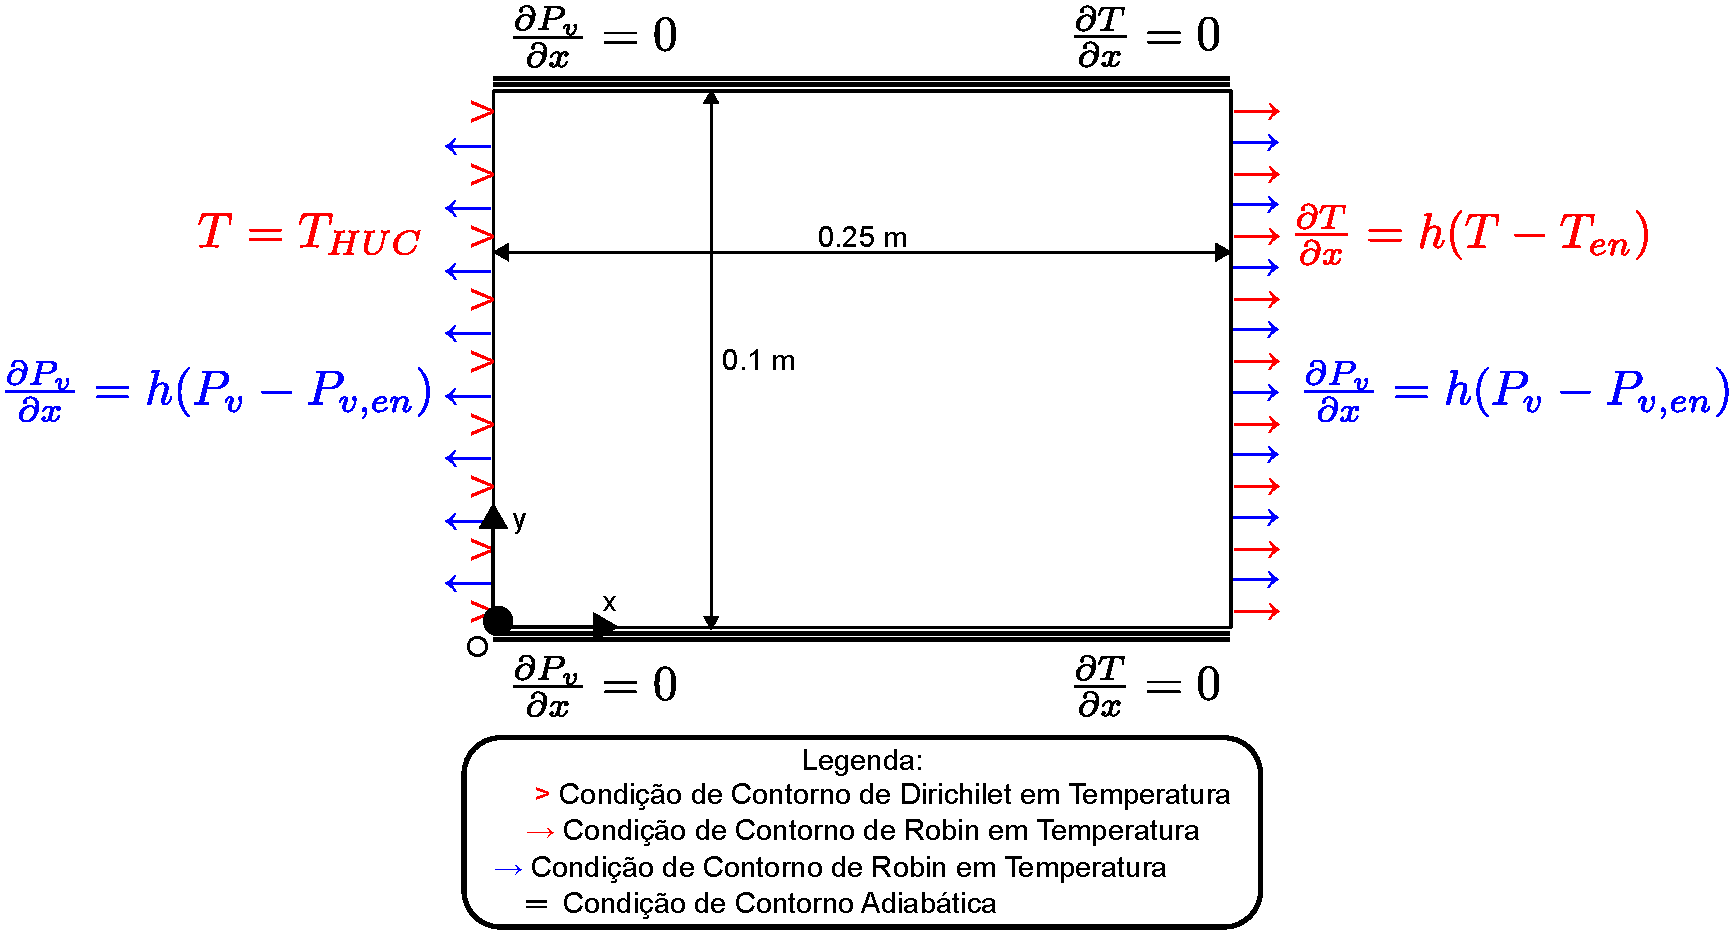
\includegraphics[width=14cm]{./figures/case.pdf}
	\caption{Esquema do caso ilustrativo apresentando as dimensões e condições de
    contorno aplicadas.  \label{fig:case}}
  \end{figure}

  \setlength{\tabcolsep}{38pt}
  
\begin{table}[]
\centering
\caption{Simulação do caso ilustrativo}
\label{tab:case_ics_bcs}
\begin{tabular}{|ll|}
\hline
\multicolumn{2}{|l|}{Discretização no espaço e no tempo}                                    \\ \hline
Espessura da parede                                          & $L_x = 25 cm$                \\
Tempo simulado                                               & $t = 25 h$                   \\
Número de elementos em $x$                                   & $n_x = 50$                   \\
Número de elementos em $y$                                   & $n_y = 20$                   \\
Incremento de tempo                                          & $\Delta t = 15 s$            \\ \hline
\multicolumn{2}{|l|}{Condições Iniciais}                                                    \\ \hline
$T(x, y, t=0)$                                               & $ 25 ^{\circ}C$              \\
$P_v(x, y, t=0)$                                             & $ 2850 N \ m^{-2} $          \\ \hline
\multicolumn{2}{|l|}{Condições de Contorno}                                                 \\ \hline
$T(x=0, y, t)$                                               & $T_{HUC}(t)$                 \\
$\frac{\partial T}{\partial x}\bigg\rvert_{x = L_x, y, t}$   & $h \ (T - T_{en})$           \\
$\frac{\partial T}{\partial y}\bigg\rvert_{x, y=0, t}$       & $0$                          \\
$\frac{\partial T}{\partial y}\bigg\rvert_{x, y=L_y, t}$     & $0$                          \\
$\frac{\partial P_v}{\partial x}\bigg\rvert_{x = 0, y, t}$   & $h_m \ (P_v - P_{v, en})$    \\
$\frac{\partial P_v}{\partial x}\bigg\rvert_{x = L_x, y, t}$ & $h_m \ (P_v - P_{v, en})$    \\
$\frac{\partial P_v}{\partial y}\bigg\rvert_{x, y=0, t}$     & $0$                          \\
$\frac{\partial P_v}{\partial y}\bigg\rvert_{x, y=L_y, t}$   & $0$                          \\ \hline
\multicolumn{2}{|l|}{Propriedades}                                                          \\ \hline
Condutividade térmica do concreto refratário, $\lambda$      & $7 W \ m^{-1} \ K^{-1}$      \\
Densidade do concreto refratário, $\rho$                     & $2200 Kg \ m^{-3}$           \\
Calor específico do concreto refratário, $C_p$               & $1100 J \ Kg^{-1} \ K^{-1}$  \\
Curvas de Sorção Isotérmica, $w$                             & Equation \ref{eq:gong_phi}           \\
Permeabilidade, $K$                                          & Equation \ref{eq:baz_perm}           \\
Permeabilidade inicial, $K_0$                                & $ 10^{-12} m \ s^{-1}$       \\
Calor específico da água, $C_w$                              & $ 4100 J \ Kg^{-1} \ K^{-1}$ \\
Coeficiente de transferência de calor, $h$                   & $ 1 W \ m^{-2} \ K^{-1}$     \\
Coeficiente de transferência de calor, $h_m$                 & $ 1 \ 10^{-^6} s \ m^{-1}$   \\
Temperatura ambiente, $T_{en}$                               & $ 25 ^{\circ}C$              \\
Pressão Parcial de vapor de água, $P_{v, en}$                & $ 2850 N \ m^{-2} $          \\
Quantidade de cimento por Kg de concreto, $w_c$              & $ 300 Kg m^{-3} $            \\
Quantidade de água inicial por Kg de concreto, $w_0$         & $ 100 Kg m^{-3} $            \\ \hline
\end{tabular}
\end{table}

    A permeabilidade, ($K$), é retirada do modelo de Bažant, que também é utilizada pelo
    trabalho de Gong. Já a sorção isotérmica ($w$) é adaptada de \ref{eq:baz_phi}
    conforme descrito por Gong e representado pela Equação \ref{eq:gong_phi}.

\begin{equation}
  \label{eq:gong_phi}
      w(P, T) =
      \begin{cases} 
      w_c \left( \frac{w_0}{c} \ \phi(P,T) \right)^{\frac{1}{m(T)}} & \phi(P, T)\leq 0.96 \\
      w_{0.96} + (\phi(P, T) - 0.96) \frac{(w_{1.04} - w_{0.96})}{(1.04-0.96)} & 0.96 < \phi(P, T) < 1.04 \\
 w_c \ \left[0.037 (\phi-1.04) + 0.3335 \left(1 - \frac{T^2}{3.6 \ 10^5}) \right) \right] & \ 1.04 \leq \phi(P, T)
      \end{cases}
\end{equation}

    O uso de tal versão se justifica pois a equação é ajustada para a
    microestrutura de um concreto refratário \cite{Gong1995a} e ao não utilizar
    da porosidade, apresenta uma maior simplicidade de uso. Provido das
    propriedades apresentadas na Tabela \ref{tab:case_ics_bcs}, da geometria e
    das condições iniciais e de contorno, basta definir o sistema de equações a
    ser resolvido.

    \subsection{Sistema de Equações}\label{mat:eqs}
    Problemas de caráter transiente são modelos matemáticos cujas variáveis de
    resposta dependem do tempo. A solução de tais problemas através de modelos
    numéricos implica em uma discretização no tempo e no espaço. Há inúmeras
    estratégias para tal tarefa, porém no presente trabalho se utilizará de uma
    discretização espacial a partir de elementos finitos e temporal a partir de
    diferenças finitas.

    Conforme já apresentado na Seção \ref{sec:bazant}, a formulação se baseia no
    balanço de massa e energia dos fluxos de uma quantidade denominada umidade
    que representa tanto a água líquida livre, adsorvida e o vapor de água. A
    forma forte do sistema é composta pelas equações de balanço derivadas de
    \ref{eq:baz_MB} e \ref{eq:baz_EB}, pelas condições iniciais e de contorno. 
    
    \subsubsection{Forma Forte}\label{mat:forte}
    No presente modelo as variáveis independentes escolhidas são a temperatura
    $T$ e a pressão nos poros, $P_v$. A apresentação da formulação do problema em
    sua forma forte será descrito levando em consideração funções não explicítas
    das variaveis independentes a fim de simplificar as expressões matemáticas.

    
    Substituindo as Equações \ref{eq:Darcy}, \ref{eq:Fourier} nas
    Equações  \ref{eq:baz_MB} e \ref{eq:baz_EB} obtém-se o problema em sua forma
    forte:  

    Equações de Conservação:
   \begin{equation}
     \label{eq:full_MB}
     \frac{\partial w}{\partial t}  = \nabla \cdot \left(\frac{K}{g} \nabla P_v \right) + \frac{\partial w_d}{\partial t} \ \text{in } \Omega
   \end{equation}

   \begin{equation}
      \label{eq:full_EB}
      \frac{\partial T}{\partial t} = C_a \ \frac{\partial w}{\partial t} +  C_w \frac{K}{g} \ \nabla P_v \cdot \nabla T + \nabla \cdot (\lambda \nabla T) \ \text{in } \Omega
   \end{equation}

   Condição de contorno de Dirichlet:
   \begin{equation}
     \label{eq:dir_bc}
    T(0, y, t) = T_{HUC}(t) \ \text{in } \Gamma_D
   \end{equation}

   Condições de contorno de Neumann:
   \begin{equation}
     \label{eq:neu_bc_T_x}
     \frac{\partial T}{\partial x}\bigg\rvert_{x = L_x, y, t} =  (T - T_{en}) \ \text{in } \Gamma_{N, T_{env}}
   \end{equation}

   \begin{equation}
     \label{eq:neu_bc_T_y}
\frac{\partial T}{\partial y}\bigg\rvert_{x, y=0, t} = \frac{\partial T}{\partial y}\bigg\rvert_{x, y=L_y, t} = 0 \ \text{in } \Gamma_{N, adi}
   \end{equation}

   
   \begin{equation}
     \label{eq:neu_bc_P_x}
     \frac{\partial P_v}{\partial x}\bigg\rvert_{x = 0, y, t} = \frac{\partial P_v}{\partial x}\bigg\rvert_{x = L_x, y, t} =  h_m \ (P_v - P_{v, en}) \ \text{in } \Gamma_{N, P_{env}}
   \end{equation}

   \begin{equation}
     \label{eq:neu_bc_P_y}
    \frac{\partial P_v}{\partial y}\bigg\rvert_{x, y=0, t}= \frac{\partial P_v}{\partial y}\bigg\rvert_{x, y=L_y, t} = 0 \ \text{in }\Gamma_{N, adi}
   \end{equation}


   
    Deve-se salientar que as derivadas temporais das curvas de sorção são
    obtidas a seguir como função das derivadas parciais das variáveis
    independentes. Tal abordagem permite expressar o problema em termos mais simples.

    \begin{equation}
      \label{eq:dwdt}
      \frac{\partial w}{\partial t} = \frac{\partial w}{\partial P_v} \frac{\partial P_v}{\partial t} + \frac{\partial w}{\partial T} \frac{\partial T}{\partial t}
    \end{equation}

    Além disso, as derivadas temporais das variáveis independentes são aproximadas
    por diferenças finitas anteriores conforme descrito pelas Equações \ref{eq:fd_P} e \ref{eq:fd_T}.

    \begin{equation}
      \label{eq:fd_P}
      \frac{\partial P_v}{\partial t} = \frac{P_v - P_v^n}{\Delta t}
    \end{equation}
    
    \begin{equation}
      \label{eq:fd_T}
      \frac{\partial T}{\partial t} = \frac{T - T^n}{\Delta t}
    \end{equation}

    Por fim, as derivadas parciais das curvas de sorção isotérmica são
    aproximadas por diferenças finitas centrais, Equações \ref{eq:fc_P} e \ref{eq:fc_T}.

    \begin{equation}
      \label{eq:fc_P}
      \frac{\partial w}{\partial P_v^n} = \frac{w(P_v^n+\delta \ P_v^n, \ T^n)- w(P_v^n- \delta \ P_v^n , \ T^n)}{2 \ \delta}
    \end{equation}

    
    \begin{equation}
      \label{eq:fc_T}
      \frac{\partial w}{\partial T^n} = \frac{w(P_v^n, \ T^n+\delta \ T^n)- w(P_v^n, \ T^n- \delta \ T^n)}{2 \ \delta}
    \end{equation}

    Onde $\delta$ é um diferencial numérico com valor $\delta = 0.0001$.

    
    \subsubsection{Forma Fraca}\label{mat:fraca}
    A forma fraca é obtida a partir da multiplicação das equações de conservação
    de massa e de energia pela função teste $\psi$ e subsequente integração
    sobre o domínio numérico. É utilizada a identidade de Green quando aplicável
    para se obter a forma fraca final.

  \begin{equation}
     \label{eq:weak_MB}
  \int_{\Omega}  \frac{\partial w}{\partial t} \ \psi \ \text{d}x =   \int_{\Omega}    \frac{K}{g} \left(  \nabla P_v \cdot \nabla  \psi \right) \ \text{d}x +   \int_{\Omega}    \frac{\partial w_d}{\partial t}  \ \psi \ \text{d}S \ +   \int_{\Gamma_{N, P_{env}}} \left( P_v \cdot \mathbf{n} \right) \ \psi \ \text{in } \Omega
   \end{equation}

   \begin{eqnarray}
     \label{eq:weak_EB}
      \int_{\Omega} \frac{\partial T}{\partial t} \ \psi \ \text{d}x &=&
                                                                         \int_{\Omega}
                                                                         C_a \
                                                                         \frac{\partial
                                                                         w}{\partial
                                                                         t} \
                                                                         \psi \
                                                                         \text{d}x
                                                                         +
                                                                         \int_{\Omega}
                                                                         C_w
                                                                         \frac{K}{g}
                                                                         \
                                                                         \nabla
                                                                         P_v
                                                                         \cdot
                                                                         \nabla
                                                                         T \
                                                                         \psi \
                                                                         \text{d}x
     \nonumber \\
                                                                         & &+ \int_{\Omega} \lambda \ \nabla T \cdot \nabla \psi \ \text{d}x + \int_{\Gamma_{T_{env}}} \left( T \cdot \mathbf{n} \right) \ \psi \ \text{d}x \ \text{in } \Omega
    \end{eqnarray}

    
    Tal sistema é fornecido à biblioteca FEniCS que converte o sistema de
    equações parciais diferenciais em um sistema linear de equações baseado nas
    funções de forma escolhidas. Esse sistema é resolvido iterativamente e o
    resultado é obtido através dos valores nodais (em cada um dos nós da malha
    que representa a discretização da geometria do problema) das variáveis de interesse.

    A seguir será delineado a estrutura do código apresentando uma clara
     correlação com cada etapa da descrição matemática.
     
    \subsection{Estrutura do script}\label{mat:script}
    O script pode ser separado nas seguintes etapas:

    \begin{itemize}
    \item Importação das bibliotecas necessárias
    \item Definição dos parâmetros de discretização temporal e espacial
    \item Definição da malha a partir da geometria
    \item Especificação das condições de contorno
    \item Definição dos espaços das funções de elementos finitos
    \item Definição das propriedades dos materiais
    \item Especificação das condições iniciais
    \item Descrição do sistema de equações em sua forma fraca
    \item Loop temporal de resolução das equações e armazenamento dos resultados 
    \end{itemize}

    Cada uma das etapas serão detalhadas e o código mostrado. O arquivo com
    todos os comandos é apresentado no Apêndice [REF].

    
    \subsubsection{Importação das bibliotecas}
    Para a simulação, apenas o pacote \mintinline[bgcolor=bg]{python}{dolfin} da biblioteca
    FEniCS é necessário. O pacote \mintinline[bgcolor=bg]{python}{datetime} é utilizado para
    contabilizar o tempo decorrido de simulação. Já os pacotes
    \mintinline[bgcolor=bg]{python}{csv} e \mintinline[bgcolor=bg]{python}{os} são importados para
    salvar as séries temporais de variáveis de interesse em uma planilha e para 
    gerenciar em qual diretório serão salvos os arquivos, respectivamente.

    \begin{minted}[
      frame=lines,
      framesep=2mm,
      baselinestretch=1.2,
      bgcolor=bg,
      fontsize=\footnotesize,
      linenos
      ]{python}

      from dolfin import *
      from datetime import datetime
      import csv
      import os
    \end{minted}
   
    \subsubsection{Definição da discretização}
    Conforme definido na Tabela \ref{tab:case_ics_bcs}, a discretização é
    definida a partir das seguintes variáveis.
    
    \begin{minted}[
      frame=lines,
      framesep=2mm,
      baselinestretch=1.2,
      bgcolor=bg,
      fontsize=\footnotesize,
      linenos
      ]{python}
      
      # Time discretization
      t = 0
      T_total = 25 * 3600
      dt = 15
      
      # Space discretization
      lx = 0.25
      ly = 0.10
      Nx = 50
      Ny = 20
    \end{minted} 

    \subsubsection{Definição da malha e das condições de contorno}
    O pacote FEniCS já vem com uma ferramenta capaz de gerar malhas em
    geometrias simplistas. Dessa forma, para definir a malha da seção retangular
    da parede do caso de estudo é simples utilizando apenas a função
    \mintinline[bgcolor=bg]{python}{RectangleMesh()}. Em seguida, cria-se um
    objeto que representa as condições de contorno através da função
    \mintinline[bgcolor=bg]{python}{MeshFunction()}, cujos argumentos definem
    qual o tipo desse contorno (face interna ou externa), a malha, e a dimensão
    do contorno (pontos para um domínio unidimensional, curvas para domínios
    bidimensionais e superfícies para domínios tridimensionais). Por fim, é
    criada uma classe para cada parede do retângulo. Tais classes são utilizadas
    para marcar uma bandeira em cada nó que pertence a tais contornos. Por fim é
    criada uma medida através da função \mintinline[bgcolor=bg]{python}{Measure()} que será utilizada na formulação da forma fraca.
    
    \begin{minted}[
      frame=lines,
      framesep=2mm,
      baselinestretch=1.2,
      bgcolor=bg,
      fontsize=\footnotesize,
      linenos
      ]{python}

      # Mesh and Boundaries Condition Definitions
      mesh = RectangleMesh(0.0, 0.0, lx, ly, Nx, Ny)

      # Boundaries
      boundaries = MeshFunction('size_t', mesh, mesh.topology().dim() - 1)
      boundaries.set_all(0)


      class left(SubDomain):
          def inside(self, x, on_boundary):
              return abs(x[0]) < DOLFIN_EPS and on_boundary
      

      class right(SubDomain):
          def inside(self, x, on_boundary):
              return abs(x[0] - lx) < DOLFIN_EPS and on_boundary


      class top(SubDomain):
          def inside(self, x, on_boundary):
              return abs(x[1] - ly) < DOLFIN_EPS and on_boundary


      class down(SubDomain):
          def inside(self, x, on_boundary):
              return abs(x[1]) < DOLFIN_EPS and on_boundary


      left = left()
      right = right()
      top = top()
      down = down()
      left.mark(boundaries, 1)
      right.mark(boundaries, 2)
      top.mark(boundaries, 3)
      down.mark(boundaries, 4)
      ds = Measure("ds", domain=mesh, subdomain_data=boundaries)
    \end{minted} 

    \subsubsection{Definição dos espaços das funções de elementos finitos}
    Uma vez definida as geometrias do problema, criam-se o espaço da função de
    elementos finitos onde residem as funções teste e as funções bases que
    aproximação as variáveis independentes do problema (a temperatura e a
    pressão). Como o problema é acoplado de maneira forte, o espaço vetorial
    deverá compreender elementos que aproximem ambas as funções e para tanto
    cria-se um espaço misto. Para tanto, é criado primeiramente um objeto que
    representa um elemento finito linear
    \mintinline[bgcolor=bg]{python}{RectangleMesh(P1)}. Em seguida define-se o
    elemento misto e o espaço de função sobre a malha usando a
    função\mintinline[bgcolor=bg]{python}{FunctionSpace()}. A partir daí é
    possível obter funções teste e funções de aproximação a partir do espaço V.  
    
     \begin{minted}[
      frame=lines,
      framesep=2mm,
      baselinestretch=1.2,
      bgcolor=bg,
      fontsize=\footnotesize,
      linenos
      ]{python}
     # Mixed element and space functions definition
     P1 = FiniteElement('P', mesh.ufl_cell(), 1)
     element = MixedElement([P1, P1])
     V = FunctionSpace(mesh, element)
     v_1, v_2 = TestFunctions(V)
     u = Function(V)
     P_v, T = split(u)
     u_n = Function(V)
     P_v_n, T_n = split(u_n)

    \end{minted} 
   
    \subsubsection{Definição das propriedades do material}
    Cada uma das propriedades são definidas através de funções definidas em
    python. A única especificidade referente ao uso da plataforma FEniCS é o uso
    de uma função própria para definir condicionais. O leitor é referenciado ao
    Anexo [REF] para visualizar o código inteiro a fim de evitar prolixidade. 

    \subsubsection{Especificação das condições iniciais}
    As condições iniciais são projetadas no espaço de elementos finitos usando a
    função \mintinline[bgcolor=bg]{python}{interpolate()}.
    
    \begin{minted}[
      frame=lines,
      framesep=2mm,
      baselinestretch=1.2,
      bgcolor=bg,
      fontsize=\footnotesize,
      linenos
      ]{python}
     
     # Initial conditions
     P_0 = P_v_inf
     P_v_n = interpolate(P_0, V.sub(0).collapse())
     T_0 = Constant(298.15)
     T_n = interpolate(T_0, V.sub(1).collapse())
    \end{minted} 

    \subsubsection{Descrição da forma fraca}
    Em seguida, a forma fraca é definida. Na presente subseção também será
    criado um objeto que representa o problema numérico a ser resolvido. A
    definição de parâmetros específicos referente ao algoritmo de resolução é
    apresentado no Apêndice [REF]. A representação é direta do problema descrito
    em \ref{mat:fraca}. A integração é apenas representada implicitamente pela
    multiplicação de cada termo pela medida volumétrica
    \mintinline[bgcolor=bg]{python}{dx} ou de contorno
    \mintinline[bgcolor=bg]{python}{ds}.

    Também se define o Jacobiano do resíduo que será utilizado no algoritmo de
    resolução através do método de Newton. Por fim, são definidos objetos que
    representam o problema numérico (\mintinline[bgcolor=bg]{python}{problem}) e o algoritmo de solução em si (\mintinline[bgcolor=bg]{python}{solver}).
    
    \begin{minted}[
      frame=lines,
      framesep=2mm,
      baselinestretch=1.2,
      bgcolor=bg,
      fontsize=\footnotesize,
      linenos
      ]{python}

     # Variational formulation in residual form
     # Mass balance equation equation
     ResP = dwdt(P_v, T, P_v_n, T_n) * v_1 * dx
     ResP += (a(P_v_n, T_n) / g) * inner(nabla_grad(P_v), nabla_grad(v_1)) * dx
     ResP += - ((w_d(T) - w_d(T_n)) / dt) * v_1 * dx
     ResP += B_w * (P_v - P_v_inf) * v_1 * (ds(1) + ds(2) + ds(3) + ds(4))


     # Energy balance equation
     ResT = rho * C_p * ((T - T_n) / dt) * v_2 * dx
     ResT += k * inner(nabla_grad(T), nabla_grad(v_2)) * dx
     ResT += - h_d * ((w_d(T) - w_d(T_n)) / dt) * v_2 * dx
     ResT += - C_a(T_n) * dwdt(P_v, T, P_v_n, T_n) * v_2 * dx
     ResT += C_w * (a(P_v_n, T_n) / g) * \
         inner(nabla_grad(P_v_n), nabla_grad(T_n)) * v_2 * dx
     ResT = ResT + (B_t * (T - T_inf) +
                   C_a(T_n) * B_w * (P_v - P_v_inf)) * v_2 * (ds(2) + ds(3))


     # Total residual
     Res = ResT + ResP

     # Jacobian
     Jac = derivative(Res, u)
     problem = NonlinearVariationalProblem(Res, u, bcs, Jac, ffc_options)
     solver = NonlinearVariationalSolver(problem)
    \end{minted} 

    \subsubsection{Loop temporal}
    Em seguida, após a definição do problema e do objeto que representa o
    algoritmo de solução cria-se um loop que deverá rodar até o tempo de
    simulação alcançar o tempo total simulado (25 h). A evolução da pressão
    máxima, da temperatura máxima e da quantidade de água livre do sistema são
    salvos em um arquivo .csv que permite sua visualização online (i.e. durante
    a simulação).

    Ao entrar no loop o tempo atual de simulação é utilizado para
    definir em qual etapa da curva de aquecimento se está. Isto define a
    temperatura na condição de contorno de Dirichlet. Em seguida é resolvido o
    sistema linear de equações. A quantidade de água livre no sistema é
    integrada ao longo do domínio e os valores do timestep anterior são
    igualados ao timestep atual. A cada dez ciclos dentro do loop os resultados
    de todo o domínio são salvos em um arquivo que pode ser visualizado através
    da plataforma Paraview [REF]. O tempo de simulação é corrigido e o ciclo se
    inicia novamente.

    Ao alcançar o tempo total de simulação o programa saí do loop, o arquivo csv
    é salvo e se calcula o tempo real gasto pela simulação.
    
     \begin{minted}[
      frame=lines,
      framesep=2mm,
      baselinestretch=1.2,
      bgcolor=bg,
      fontsize=\footnotesize,
      linenos
      ]{python}
     f = open(dir_ + '/time_series.csv', 'w')
     writer = csv.writer(f, delimiter='\t')
     startTime = datetime.now()
     while t <= T_total:

         print('Progress: ' + str(round(t / T_total * 100, 2)) + '%')
     
         # Solve non-linear problem
         T_huc.t = t
         if t < 5 * 3600:
             T_huc.rate = 50
             T_huc.T_0 = 298.15
         elif (t > 5 * 3600) & (t < 10 * 3600):
             T_huc.rate = 0
             T_huc.T_0 = 298.15 + 250
         elif (t > 10 * 3600):
             T_huc.rate = 30
             T_huc.t_0 = 15.833 * 3600
             T_huc.T_0 = 298.15 + 250

         n, conv = solver.solve()

         # integration over domain of water quantity
         wat = assemble((w(P_v_n, T_n)) * dx,
                        form_compiler_parameters=ffc_options)
         w_domain.append(wat)
         convergence.append(n)
         time.append(t)

         # Update solution with last computed value
         (_P, _T) = u.split(True)
         P_v_n.vector()[:] = _P.vector()
         T_n.vector()[:] = _T.vector()
         P_v_max = max(P_v_n.vector()[:]) / 1e6
         P_v_min = min(P_v_n.vector()[:]) / 1e6
         T_max = max(T_n.vector()[:])
         T_min = min(T_n.vector()[:])

         writer.writerow([t, H, wat, n, T_max, P_v_max])

         if (nt % freq_out == 0):
             _P.rename("Pressure [Pa]", "P_v")
             _T.rename("Temperature [K]", "T")
             filex.write(_P, t)
             filex.write(_T, t)

         nt += 1
         t += dt
     # End loop over time steps
     f.close()
     time_delta = datetime.now() - startTime
     print('Simulation time: ', str(time_delta))
    \end{minted} 
   
    \subsection{Pós-processamento}
    O pós processamento se dá através de dois tipos de dados principais, são
    eles o arquivo csv que tem como objetivo dar um indicativo qualitativo da
    convergência correta da simulação (isto é, se o resultado é condizente, se a
    temperatura de aquecimento é obedecida, se a pressão máxima é um valor
    coerente ou se a quantidade de água está seguindo o comportamento já
    esperdo), e os dados nodais de todo o domínio.

    Os dados do domínio são os mais importantes porém resultam em arquivos
    pesados (dependendo do refinamento da malha e do tamanho do incremento de
    tempo). Portanto dependendo da simulação o intervalo de registro dos dados
    pode ser maior ou menor. Análises qualitativas são realizadas usando o
    Paraview enquanto análises quantitativas, descritas em termos de gráficos da
    evolução de propriedade em diferentes posições ou de perfis térmicos em
    diferentes tempos, são obtidos por rotinas em Python.



    
%%% Local Variables:
%%% mode: latex
%%% TeX-command-extra-options: "-shell-escape"
%%% TeX-master: "TCC-Secagem"
%%% End:
